\begin{figure}[h]
    \centering
    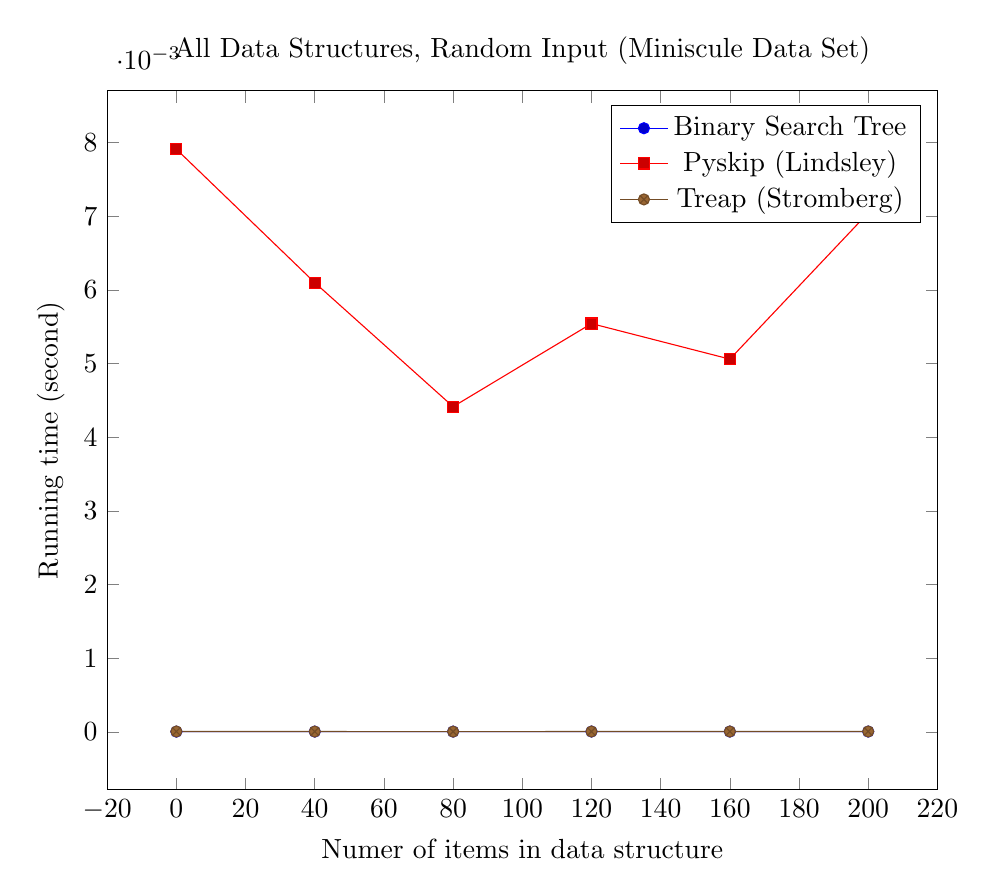
\begin{tikzpicture}
        \begin{axis}[
            xlabel={Numer of items in data structure},
            ylabel={Running time (second)},
            title={All Data Structures, Random Input (Miniscule Data Set)},
            width=\textwidth
        ]
		\addplot coordinates {
			(0, 4.065867046147611e-06)
			(40, 4.577865118625489e-06)
			(80, 4.818805388026766e-06)
			(120, 5.180215792128726e-06)
			(160, 4.879040455377064e-06)
			(200, 5.150098258453577e-06)
		};
		\addplot coordinates {
			(0, 0.007908442697627516)
			(40, 0.006098077748413156)
			(80, 0.004414537733504975)
			(120, 0.005541867136500134)
			(160, 0.005059414364557657)
			(200, 0.00704452124415531)
		};
		\addplot coordinates {
			(0, 6.384917139357071e-06)
			(40, 5.57174372985969e-06)
			(80, 4.397159916535997e-06)
			(120, 5.752448931772846e-06)
			(160, 5.993389201464084e-06)
			(200, 6.2945645382228575e-06)
		};
        \legend{Binary Search Tree, Pyskip (Lindsley), Treap (Stromberg)}
        \end{axis}
    \end{tikzpicture}
    \caption{Average of 10 operations, benchmarked every 40, starting at 0. Median of 11 runs.}
\end{figure}